\section{Applications}
%%%%%%%%%%%%%%%%%%%%%%%%%%%%%%%%%%%%%%%%%%%%%%%%%%%%%%%%%%%%

What are all the useful things to do when rewriting code?  Duncan's very
helpful docs here http://www.omegahat.net/CodeDepends/design.pdf give a
handful of reasons.

Other things that I can think of:

Identification and elimination of dead code.

- Given a big ugly script, pull out the minimal set of code to produce a
  final result. For example, everything needed to make `plot(finalresult)`.
- Parse Rhistory to find the minimal set of code to reproduce a result.
- Separate single scripts into multiple scripts if they actually have two
  independent sequences of computation.

These ideas stay much closer to the syntax and language of R compared to
what Nick is doing.

I've been considering this for the purpose of analyzing, accelerating and
optimizing essentially single scripts. But how important is this generally?
It only matters if someone's script runs slow. Probably this mostly happens
due to one large computation. If they're doing two large and independent
computations in one script shouldn't that be two scripts? But these tools
should be able to split them up at that level if I ask them to.

Remove all objects as soon as they're finished being used in the script. If
creating many large intermediate objects this could help with not using
excessive memory.

\section{Detecting Parallelism}
%%%%%%%%%%%%%%%%%%%%%%%%%%%%%%%%%%%%%%%%%%%%%%%%%%%%%%%%%%%%

Not sure how to generally detect where the possibilities for
parallel are. In a simple case of k obvious threads with one common
ancestor and common child there is an obvious option:

Remove the common ancestor and child and select the k disjoint subgraphs
between them.

Alternatively:

1. Start at the top of the graph, and move down until one node has
multiple children. Gather those child threads into 2 groups.
2. Same thing starting at the bottom.

The most straightforward thing to do right now is take a more complex
graph, say something like this:

\centerline{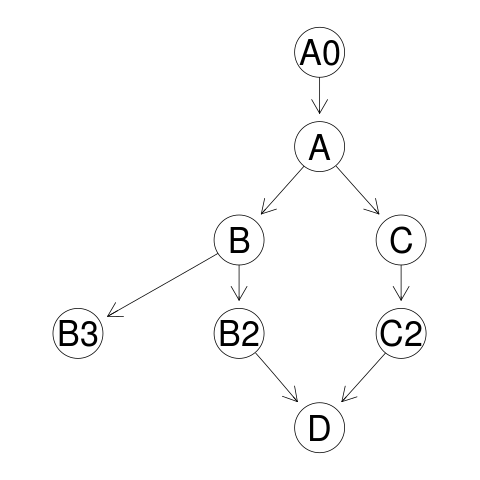
\includegraphics{../codedepends/larger_graph.png}}


And attempt to collapse the structure into one where the parallel threads
become obvious:

\centerline{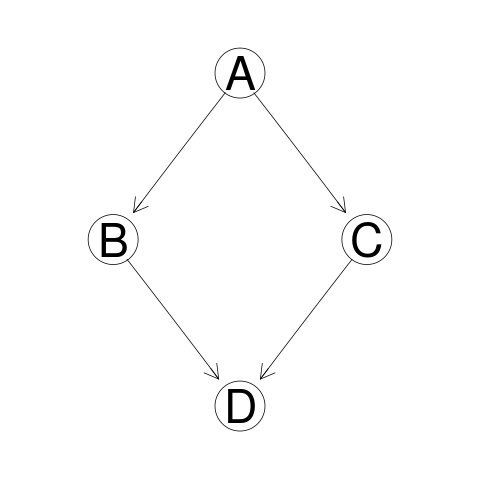
\includegraphics{../codedepends/simple_graph.png}}

The essential part for the multiprocessing is to have many "adjacent"
threads (is there a correct graph term for this?)
Optionally the adjacent threads can share a common parent and or child
nodes.


\section{Implementation}
%%%%%%%%%%%%%%%%%%%%%%%%%%%%%%%%%%%%%%%%%%%%%%%%%%%%%%%%%%%%

At first I iterated over the blocks of code and gathered dependency info as
I went along. But then I switched the implementation to focus on the variables
themselves to make my code easier to reason about. It should be slightly
more efficient, but that's not really a concern yet.

I consider updates of a list to be changes to the global list variable.
Thus something like the following redefines x every time. 

\begin{verbatim}
    x = list()
    x$a = f(...)
    x$b = g(...)
\end{verbatim}
 
This is easy and safe to do, but it might be inefficient if \texttt{f, g}
are expensive functions, because they could be run in parallel. An
alternate way is to think of \texttt{x\$a} as a variable that depends on
the original \texttt{x}. But adding details like these isn't worth it to me
now, because it's not core to what I'm trying to accomplish.

Detail- Calls to \texttt{library} need to make it to the top of the graph. Maybe in
general I can adopt the \LaTeX idea of a preamble, or setup code. But what else would go
there besides library?

It would be nice if I could look at the R global environment, then
look at an updated environment after running a line of code and take this
as the update. 

\newpage
\newpage

\section{Chunking}

IDEA: nested parallelism- how to do it? If you hard code it in you're
stuck.

The task based parallelism isn't as relevant to how people use R (and other
languages) for data processing. Instead
lets think more about chunking and data parallelism. 

Parallelism introduces additional overhead on top of what dynamic languages
already incur. A general strategy to minimize this overhead is to ``chunk''
the computations. For example, given 1000 parallel operations one might
partition these into chunks of size 100 so that they become 10 parallel
tasks \cite{matloff2015parallel}.

I can take the code in \cite{matloff2015parallel} and see how changing the
chunk sizes affects the run time. I could also do this with Python's dask.
The goal is to draw general conclusions about which chunk sizes work best
based on the amount of computation.

It would be nice to run just a couple in serial on the master process and
make principled decisions about how to run based on these results. For
example:
\begin{itemize}
    \item Is it worth it to run in parallel?
    \item Should we chunk? What should the chunk sizes be?
    \item Reverse the order for better load balancing?
    \item Dynamic or static scheduling?
\end{itemize}

Usually none of these are known ahead of time.  They also depend on the
particular problem.  The only way to know if a chunking scheme will work is
to experiment with a similar problem, then check expectations for the next
one. I also expect that they vary across different machines.

The book mentions using large chunks in the beginning followed by small
chunks for superior load balancing.

Programming in the RDSM package conceptually is very similar to OpenCL on
the GPU. You allocate memory and send it to the workers, then update it in
place based on thread IDs. This is quite different than normal functional
R. I wonder if we could "translate" regular R into this style of
programming?

TODO: Come up with application where I need all this!! How about computing
graphs from Euclidean space like with James' application? It would be nice
for the QE to have something that he's familiar with and invested in.


